\chapter{Funktionsweise und Aufbau}
\label{ch:Aufbau}

Der Gestikulaser gehört weder zu den gerätebasierten, noch zu den kamerabasierten Gestenerkennungssystemen. Seine Funktionsweise ist aber mit der von kamerabasierten Gestenerkennungssystemen vergleichbar. Statt jedoch den Nutzer bei seinen Bewegungen zu beobachten und davon Aufnahmen zu machen, die in einem nachfolgenden Schritt von einem Computer analysiert werden, detektiert der Gestikulaser mit Hilfe von Photodioden die infraroten Lichtsignale einer LED-Quelle, die von der Hand des Nutzers reflektiert werden, während er eine Geste ausführt. Die an den Photodioden gemessenen Photoströme werden anschließend an einen Computer weitergeleitet und dort in einer von uns entwickelten Software weiterverarbeitet, welche mit Hilfe eines zuvor antrainierten künstlichen neuronalen Netzes die tatsächliche Handgeste erkennt. Nach der Auswertung wird die erkannte Geste genutzt, um mit einem zuvor hinterlegten Befehl ein beliebiges Endgerät anzusteuern. Dieser Ablauf ist in \reffig{fig:AblaufGestikulaser} schematisch dargestellt.
\begin{figure}[h]
	\centering
	\includegraphics[width=15cm]{../figures/AblaufGestikulaser2.jpg}
	\caption{Schmatische Darstellung der Gestenerkennung mit dem Gestikulaser.}
	\label{fig:AblaufGestikulaser}
\end{figure} \\
Der Gestikulaser besteht aus mehreren Modulen, die über USB-Steckverbindungen mit einander verbunden werden können. Jedes Steckmodule besteht aus einer einzelnen kleinen Box, in welche die Elektronik integriert ist. Das Herzstück des Gestikulasers bildet der \textit{Oktokommander} (siehe auch \refsec{sec:Oktokommander}), der zugleich die Schnittstelle zu dem Computer bereitstellt, in dem die eigentliche Gestenerkennung erfolgt. An ihn können in der aktuellen ersten Version bis zu sieben \textit{Detektormodule} (siehe auch \refsec{sec:Detektormodul}) angesteckt werden. Auf jedem dieser Module befinden sich vier Photodioden, um das reflektierte Licht zu messen. 
\begin{figure}[h]
	\centering
	\includegraphics[width=9cm]{../CAD_Bilder/Gestikulaser_raytraced_2.png}
	\caption{Aufsicht auf das CAD Modell des Gestikulasers. In der ersten Version können bis zu sieben Detektormodule (außen) an den Oktokommander (innnen) angesteckt werden. Eine Erweiterung um weitere Detektormodule ist technisch möglich.}
	\label{fig:Gestikulaser}
\end{figure}

% -------------------------------------------------------------------------------------- %

\section{Oktokommander}
\label{sec:Oktokommander}

Die zentrale Elektronikeinheit des Oktokommanders bildet ein Arduino Micro, der alle Komponenten des elektrischen Schaltkreises, wie die Detektormodule und die Photodioden, über einen I2C Bus ansteuert. Für die Übertragung der Sensordaten zum Computer ist er über ein Datenkabel mit einem Computer verbunden, wodurch zugleich die Stromversorgung des Schaltkreises sichergestellt wird. Die I2C Bus Verbindung benötigt lediglich 2 Pins auf dem Arduino, SDA für die eigentliche Datenverbindung und SCL für den vom Arduino vorgegebenen Takt. Die Ansteuerung jedes einzelnen Sensors erfolgt über eine, im System einzigartige, Hardware Adresse (I2C-Adresse). Mit den eingesetzten I2C AD-Wandler (ADS1015) lassen sich maximal 4 I2C Adressen erzeugen. Jeder I2C AD-Wandler verfügt dabei über 4 Pins, über die die verschiedenen Sensoren angesteuert und ausgelesen werden können. Auf diese Weise könnten maximal 16 Photodioden für die Detektion der von der Hand des Nutzers reflektierten Infrarot Strahlung der LEDs verwendet werden. Um ein Rahmenwerk zur Erkennung von möglichst vielen verschiedenen Gesten zu schaffen, ist eine große Anzahl von Photodioden nützlich. Aus diesem Grund wird ein zusätzlicher I2C Multiplexer (TCA9548A) in den Oktokommander eingebaut. Der Multiplexer erhöht die Anzahl der verwendbaren I2C AD-Wandler und damit letztendlich auch die Anzahl der verwendbaren Photodioden, indem er die erzeugten Adressen multiplext. Der verwendete Multiplexer kann 8 verschiedene Adressen erzeugen, die sich nicht mit den Adressen der I2C AD-Wandler überlagern und besitzt je 8 SDA und SCL Pins, an denen die I2C AD-Wandler angeschlossen werden. In der Theorie lassen sich damit bis zu 1024 Sensoren über einen Mikrocontroller ansteuern. Für den Gestikulaser beschränken wir uns auf die Verwendung eines einzelnen Multiplexers, wodurch wir bis zu 128 Photodioden zur Detektion der reflektierten Strahlung verwenden können. 
\begin{figure}[H]
	\centering
	\includegraphics[scale=0.5]{../figures/oktokommander2.jpg}
	\caption{Schematischer Aufbau des Oktokommanders bestehend aus einem Arduino einem I2C Multiplexer, einem I2C AD-Wandler und einer Verstärkerschaltung.}
	\label{fig:SchaltungOktokommander}
\end{figure}
\noindent
Eine schematische Übersicht über die Verschaltung der im Oktokommander untergebrachten Elektronik ist in \reffig{fig:SchaltungOktokommander} dargestellt. Im Folgenden wird der Aufbau des Oktokommanders näher erläutert.


\subsubsection*{Konstruktion}
Die Unterbringung der Elektronik im Oktokommander erfolgt über drei sogenannte \textit{Stages}. Die Stages werden im Oktokommander übereinander angeordnet. Stage 1 ist in \reffig{fig:OktoStage1} dargestellt. Es handelt sich dabei um eine Platine, auf der der Arduino Micro, der I2C Multiplexer, ein I2C AD-Wandler, eine Verstärkerschaltung, die Stromversorgung und sieben female USB-2A-Schnittstellen zur Verbindung mit den Detektormodulen angebracht sind. Zugleich bildet sie die unterste Elektronikeinheit des Oktokommanders.
\begin{figure}[H]
	\centering
	\includegraphics[width=9cm]{../CAD_Bilder/OktagonElektronik_Stage1_raytraced.png}
	\caption{Stage 1 des Oktokommanders, auf der die wichtigsten Elektronik Bauteile untergebracht sind.}
	\label{fig:OktoStage1}
\end{figure}
\noindent
Die LED-Einheit zur Lichterzeugung wird auf einer weiteren Plattform befestigt, die über der ersten Stage positioniert wird. Diese zweite Stage ist in \reffig{fig:OktoStage2} dargestellt. Die LED-Einheit besteht aus vier LEDs, die zusammen mit Parabolzylindern auf einen Kühlkörper geklebt werden. Die Parabolzylinder sollen den Abstrahlungswinkel der LED reduzieren, um eine höhere Intensität auf der zu detektierenden Fläche zu erreichen. Zudem befinden sich die LED-Treiber auf dieser Stage, die eine externe Stromversorgung der LEDs durch ein Netzteil ermöglichen. Die Aufnahme der LED-Einheit besteht aus einer dünnen Aluminiumplatte für den Wärmeabtransport. Die Bohrungen in der Aluminiumplatte dienen lediglich zur Durchführung der Kabel zur unteren Stage 1.
\begin{figure}[H]
	\centering
	\includegraphics[width=9cm]{../CAD_Bilder/OktagonElektronik_Stage2_raytraced.png}
	\caption{Stage 2 des Oktokommanders mit den Infrarot-LEDs, die im Betrieb die Hand des Nutzers anstrahlen.}
	\label{fig:OktoStage2}
\end{figure}
\newpage
\noindent
Die oberste Stage 3 trägt vier Photodioden. Das additiv aus umweltfreundlichen PLA-Kunststoff gefertigte Bauteil ist in \reffig{fig:OktoStage3} dargestellt.
\begin{figure}[H]
	\centering
	\includegraphics[width=9cm]{../CAD_Bilder/OktagonElektronik_Stage3_raytraced.png}
	\caption{Stage 3 des Oktokommanders, auf der vier Photodioden untergebracht sind, damit auch Reflexionen nahe des Zentrums des Gestikulasers detektiert werden können.}
	\label{fig:OktoStage3}
\end{figure}
\noindent
Die drei Stages werden im Gehäuse des Oktokommanders aufgenommen. In \reffig{fig:OktoZusammenbau} ist das Gehäuse mit dem Deckel und der Elektronik des Oktokommanders dargestellt. Der Deckel und das Gehäuse des Oktokommanders werden ebenfalls additiv aus PLA-Kunststoff gefertigt.
\begin{figure}[H]
	\centering
	\includegraphics[width=12cm]{../CAD_Bilder/Oktokommander_raytraced.png}
	\caption{Explosionsdarstellung des Oktokommanders.}
	\label{fig:OktoZusammenbau}
\end{figure}


% -------------------------------------------------------------------------------------- %


\section{Detektormodul}
\label{sec:Detektormodul}

Die Hauptaufgabe der Detektormodule ist es, die Elektronik bereitzustellen, die zur Detektion der von der Hand des Nutzers reflektierten Infrarot-Strahlung benötigt wird. Aus diesem Grund enthält jedes Detektormodul vier Photodioden, eine Verstärkerschaltung, einen I2C AD-Wandler und einen USB-2A Stecker. Über den USB-2A-Stecker kann das Detektormodul an eine beliebige freie Stelle im Oktokommander angesteckt werden. Der USB-Stecker ist direkt mit dem I2C AD-Wandler verkabelt, der ebenfalls mit der Verstärkerschaltung verbunden ist. Die von den Photodioden bei Lichtdetektion ausgegebenen Photoströme werden durch diese Verstärkerschaltung verstärkt und in die Datenleitung des I2C Multiplexers eingespeist. Die Verstärkerschaltung wird im nächsten Abschnitt genauer erläutert.


\subsubsection*{Auslegung der Verstärkerschaltung}
Die Verstärkerschaltung besteht aus zwei sogenannten Transimpedanzverstärkern. Diese setzen sich zusammen aus einem Operationsverstärker vom Typ LM358, je zwei Widerständen und Kondensatoren, sowie zwei Infrarot-Photodioden. Eine schematische Darstellung des Transimpedanzverstärkers ist in \reffig{fig:Transimpedanz} dargestellt.
\begin{figure}[H]
	\centering
	\includegraphics[scale=0.75]{../figures/Transimpedanz.png}
	\caption{Schematische Darstellung des Transimpedanzverstärkersystems im Detektormodul}
	\label{fig:Transimpedanz}
\end{figure}
\noindent
Die Photodiode fungiert darin als Konstantstromquelle, welche einfallende Photonen in einen geringen elektrischen Strom umwandelt. Mit Hilfe des Widerstandes $R_1$ und des Kondensators $C_1$ kann der Operationsverstärker (LM358) eine vom Mikrocontroller verarbeitbare Spannung ausgeben. Wichtig ist hier die möglichst genaue Wahl der Kapazität $C_1$, ohne die das System anfangen würde zu Schwingen. Es gilt:
\begin{align*}
	C_1 = \sqrt{\frac{C_I}{R_1 \cdot GBP}}
\end{align*}
Hierbei steht $GBP$ für \textit{Gain Bandwidth Product}. Das ist diejenige Frequenz, bei der keine Verstärkung mehr stattfindet. Sie ist somit die Obergrenze für einen praktikablen Einsatz des Systems. Für den Operationsverstärker LM358 ist das $GBP$ mit $\unit[1]{MHz}$ im Datenblatt angegeben. $C_I$ ist die Summe der beiden Sperrschichtkapazitäten der Photodiode und des Operationsverstärkers. Typische Anwendungsgrößen für $R_1$ liegen bei etwa $\unit[1]{M\Omega}$. Der Arbeitsbereich des Verstärkersystems beschränkt sich durch aktive Bauelemente auf einen bestimmten Frequenzbereich. Dieser lässt sich wie folgt berechnen:
\begin{align*}
	f_{\unit[3]{dB}} = \sqrt{\frac{GBP}{2\pi \cdot R_1 \cdot C_I}}
\end{align*}
Für unser System liegt die Bandbreite bei etwa $\unit[73]{kHz}$, was auch die Grenzfrequenz des Verstärkersystems ist. Die Grenzfrequenz ist diejenige Frequenz, bei der die Verstärkung auf den $\frac{1}{\sqrt{2}}$-fachen Wert der maximalen Verstärkung gesunken ist und bei der die Hälfte der maximalen Leistung an einen rein Ohm'schen Verbraucher abgegeben wird.


\subsubsection*{Konstruktion}
Die wesentlichen Bestandteile des Detektormoduls sind eine Platine, die die Elektronik aufnimmt, und eine weitere Stage für die Photodioden zur Detektion des reflektierten Lichts. Auch hier werden, ähnlich wie beim Oktokommander, die Stages übereinander angeordnet. In \reffig{fig:DetektorStage1} ist Stage 1 des Detektormoduls dargestellt. Dabei handelt es sich um eine Platine mit dem male USB-Stecker, dem I2C AD-Wandler und der Verstärkerschaltung.
\begin{figure}[H]
	\centering
	\includegraphics[width=9cm]{../CAD_Bilder/DetektorElektronik_Stage1_raytraced.png}
	\caption{Stage 1 des Detektormoduls, bestehend aus einem I2C Expander und einer Verstärkerschaltung. Die Verstärkerschaltung ist nicht abgebildet.}
	\label{fig:DetektorStage1}
\end{figure}
\noindent
Darüber wird die zweite Stage angeordnet. Diese additiv aus PLA-Kunststoff gefertigte Stage erlaubt die Unterbringung der vier Photodioden und ist in \reffig{fig:DetektorStage2} dargestellt. Vom Aufbau her ist sie vergleichbar mit Stage 3 des Oktokommanders.
\begin{figure}[H]
	\centering
	\includegraphics[width=9cm]{../CAD_Bilder/Detektormodul_Stage2_raytraced.png}
	\caption{Stage 2 des Detektormoduls zur Unterbringung der Photodioden.}
	\label{fig:DetektorStage2}
\end{figure}
\noindent
Das vollständige Detektormodul ist in \reffig{fig:DetektorZusammenbau} dargestellt. Auch das Gehäuse und der Deckel des Detektormoduls werden additiv aus PLA-Kunststoff gefertigt.
\begin{figure}[H]
	\centering
	\includegraphics[width=11cm]{../CAD_Bilder/Detektormodul_raytraced.png}
	\caption{Explosionsdarstellung des Detektormoduls.}
	\label{fig:DetektorZusammenbau}
\end{figure}
\noindent
Aktuell bietet der Oktokommander Anschlüsse für die Verbindung mit bis zu sieben Detektormodulen. Zusammen bilden der Oktokommander und die Detektormodule die Hardware des Gestikulasers. Der Zusammenbau der Detektormodule mit dem Oktokommander ist \reffig{fig:GestikulaserModular} und \reffig{fig:GestikulaserKombiniert} dargestellt.
\begin{figure}[h]
	\centering
	\includegraphics[width=9cm]{../CAD_Bilder/Gestikulaser_raytraced_4.png}
	\caption{Die Detektormodule können über USB Steckverbindungen mit dem Oktokommander verbunden werden.}
	\label{fig:GestikulaserModular}
\end{figure}
\begin{figure}[h]
	\centering
	\includegraphics[width=9cm]{../CAD_Bilder/Gestikulaser_raytraced.png}
	\caption{CAD Modell des fertigen Gestikulasers, bestehend aus dem Oktokommander und sieben angeschlossenen Detektormodulen.}
	\label{fig:GestikulaserKombiniert}
\end{figure}


% -------------------------------------------------------------------------------------- %

\section{Software}
\label{sec:Software}

Die Software des Gestikulasers ist für die Zuordnung der Gesten zuständig. Die von den Detektormodulen gemessenen Reflektionsmuster werden an den Mikrocontroller im Oktokommander und von da aus an einen Computer weitergeleitet, wo sie verarbeitet werden. Bei der dazu eingesetzten Software wurde komplett auf open-source verfügbare Programme und Bibliotheken gesetzt. Der Code auf den Microcontrollern wurde mit Hilfe der \href{https://www.arduino.cc/en/Main/Software}{\texttt{Arduino IDE}} entwickelt. Die Verarbeitung am Computer erfolgt mit Hilfe von \texttt{Python} Skripten. Für den Machine Learning Teil wurde die \href{https://www.tensorflow.org/}{\texttt{TensorFlow}\texttrademark} Bibliothek verwendet. Die Software kann in zwei Teile unterteilt werden, die im Folgenden genauer erläutert werden.

\subsubsection*{Trainingsphase}
Der erste Teil der Software kommt während der Trainingsphase zum Einsatz. Hier werden die von den Photodioden gemessenen Daten aus dem Microcontroller im Oktokommander zunächst ausgelesen und gemeinsam mit einem Label, das die gerade aufgenommenen Geste codiert, in eine Datei geschrieben. Die auf diese Weise gesammelten Daten werden dann im nächsten Schritt verwendet, um ein mathematisches Modell zu erstellen. Das Modell wird dann im Live-Betrieb angewendet, um die vom Nutzer durchgeführte Geste, einer der bekannten Gesten zuzuordnen. Angenommen es stehen Daten von $N$ Photodioden zur Verfügung, dann können diese Daten in dem Vektor $x\in \mathbb{R}^N$ zusammengefasst werden. Für den Anfang soll ein Modell entwickelt werden, welches einem beliebigen gemessenen Datensatz $x$ eine der $m$ vordefinierten Gesten $G_1 , ... , G_m$ zuordnet. Dazu stellt der Nutzer vor Aufzeichnung der Daten in dem Python Skript ein, was für eine Geste $G_j$ er als nächstes aufnehmen will. Nachdem für jede Geste ausreichend Daten aufgenommen wurden, kann als nächstes das mathematische Modell erstellt werden, um die Sensordaten zu verarbeiten. Ziel ist es, ein gegebenes Datum $x_i$, das den im Live-Betrieb gemessenen Photoströmen der verschiedenen Photodioden entspricht, eindeutig einer Geste $G_j$ zuzuordnen. Damit Datum $x_i$ der Geste $G_j$ zugeordnet wird, muss die Bedingung 
\begin{align*}
	p(G_j | x_i) \geq p(G_k | x_i) \quad \forall k = 1,...,m \quad k \neq j
\end{align*}
erfüllt sein. Dabei ist $p(G_j | x_i)$ die bedingte Wahrscheinlichkeit für Geste $G_j$ gegeben die Photomessdaten $x_i$. Diese Bedingung lässt sich leicht überprüfen, allerdings ist die bedingte Wahrscheinlichkeit $p(G | x)$ unbekannt. Aus diesem Grund wird ein künstliches neuronales Netz mit Hilfe der zuvor aufgezeichneten Daten $(x,G) \in \mathbb{R}^N \times \mathbb{R}$ trainiert, das die unbekannte bedingte Wahrscheinlichkeit $p(G | x)$ annähert. Der Aufbau und das Training des neuronalen Netzes erfolgen mit Hilfe vordefinierter Methoden von \texttt{TensorFlow}\texttrademark. Nach erfolgreich abgeschlossenem Training wird das neuronale Netz in eine Datei exportiert und kann im Live-Betrieb verwendet werden.

\subsubsection*{Live-Betrieb}
Im Live-Betrieb wird das zuvor trainierte Modell verwendet, um die nun unbekannten Reflektionsmuste einer bekannten Geste zuzuordnen. Nachdem die gemessenen Daten einer Geste zugeordnet wurden, wird der mit dieser Geste verknüpfte Steuerungsbefehl bestimmt und an das angeschlossene Endgerät weitergeleitet. Dieser Ablauf ist schematisch in \reffig{fig:AblaufSteuerung} dargestellt.

\begin{figure}[h]
	\centering
	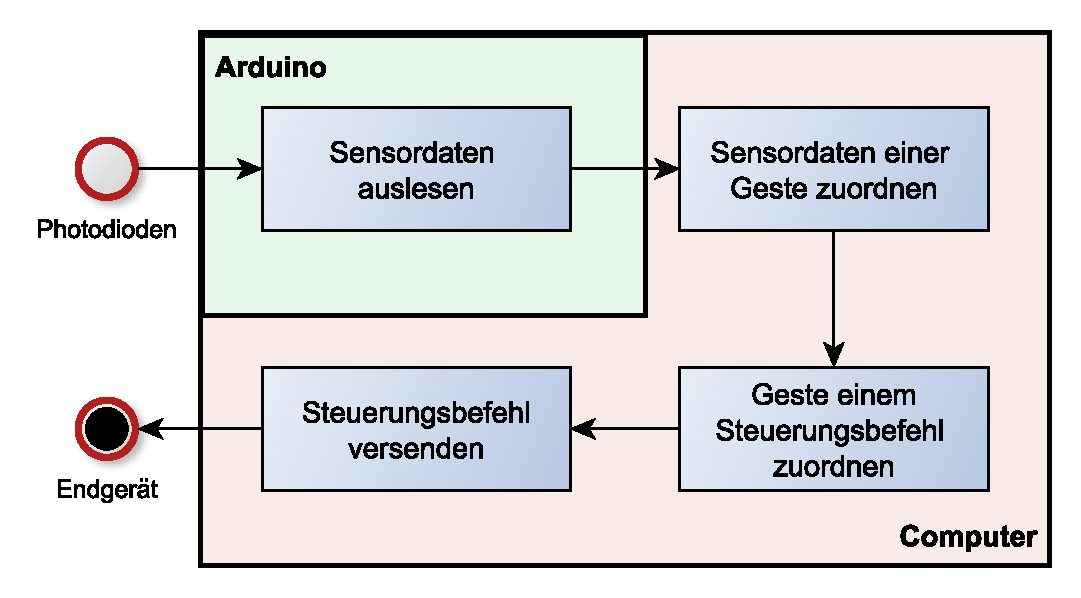
\includegraphics[scale=0.75]{../figures/AblaufSteuerung.pdf}
	\caption{Ablaufdiagramm der Software im Live-Betrieb: Die aus dem Microcontroller ausgelesenen Sensordaten werden zur Verarbeitung an das Python Skript übergeben, wo sie einer Geste und diese einem Steuerbefehl zugeordnet wird. Dieser Steuerungsbefehl wird schließlich an das anzusteuernde Endgerät weitergegeben.}
	\label{fig:AblaufSteuerung}
\end{figure}